% THIS IS SIGPROC-SP.TEX - VERSION 3.1
% WORKS WITH V3.2SP OF ACM_PROC_ARTICLE-SP.CLS
% APRIL 2009
%
% It is an example file showing how to use the 'acm_proc_article-sp.cls' V3.2SP
% LaTeX2e document class file for Conference Proceedings submissions.
% ----------------------------------------------------------------------------------------------------------------
% This .tex file (and associated .cls V3.2SP) *DOES NOT* produce:
%       1) The Permission Statement
%       2) The Conference (location) Info information
%       3) The Copyright Line with ACM data
%       4) Page numbering
% ---------------------------------------------------------------------------------------------------------------
% It is an example which *does* use the .bib file (from which the .bbl file
% is produced).
% REMEMBER HOWEVER: After having produced the .bbl file,
% and prior to final submission,
% you need to 'insert'  your .bbl file into your source .tex file so as to provide
% ONE 'self-contained' source file.
%
% Questions regarding SIGS should be sent to
% Adrienne Griscti ---> griscti@acm.org
%
% Questions/suggestions regarding the guidelines, .tex and .cls files, etc. to
% Gerald Murray ---> murray@hq.acm.org
%
% For tracking purposes - this is V3.1SP - APRIL 2009

\documentclass{acm_proc_article-sp}

\hyphenation{Data-Series Map-Reduce Network-Module Grep-Module Sort-Module}

\newenvironment{mylisting}
{\begin{list}{}{\setlength{\leftmargin}{1em}}\item\scriptsize\bfseries}
{\end{list}}

\newenvironment{mytinylisting}
{\begin{list}{}{\setlength{\leftmargin}{1em}}\item\tiny\bfseries}
{\end{list}}



\begin{document}
\title{Efficient Data-Intensive Computing}
%\title{Efficient Data-Intensive Computing\titlenote{(Does NOT produce the
%permission block, copyright information nor page numbering). For use with
%ACM\_PROC\_ARTICLE-SP.CLS. Supported by ACM.}}
%\subtitle{Do we want a subtitle?
%\titlenote{A full version of this paper is available as
%\textit{Author's Guide to Preparing ACM SIG Proceedings Using
%\LaTeX$2_\epsilon$\ and BibTeX} at
%\texttt{www.acm.org/eaddress.htm}}}
%
% You need the command \numberofauthors to handle the 'placement
% and alignment' of the authors beneath the title.
%
% For aesthetic reasons, we recommend 'three authors at a time'
% i.e. three 'name/affiliation blocks' be placed beneath the title.
%
% NOTE: You are NOT restricted in how many 'rows' of
% "name/affiliations" may appear. We just ask that you restrict
% the number of 'columns' to three.
%
% Because of the available 'opening page real-estate'
% we ask you to refrain from putting more than six authors
% (two rows with three columns) beneath the article title.
% More than six makes the first-page appear very cluttered indeed.
%
% Use the \alignauthor commands to handle the names
% and affiliations for an 'aesthetic maximum' of six authors.
% Add names, affiliations, addresses for
% the seventh etc. author(s) as the argument for the
% \additionalauthors command.
% These 'additional authors' will be output/set for you
% without further effort on your part as the last section in
% the body of your article BEFORE References or any Appendices.

\numberofauthors{2} %  in this sample file, there are a *total*
% of EIGHT authors. SIX appear on the 'first-page' (for formatting
% reasons) and the remaining two appear in the \additionalauthors section.
%
\author{
% You can go ahead and credit any number of authors here,
% e.g. one 'row of three' or two rows (consisting of one row of three
% and a second row of one, two or three).
%
% The command \alignauthor (no curly braces needed) should
% precede each author name, affiliation/snail-mail address and
% e-mail address. Additionally, tag each line of
% affiliation/address with \affaddr, and tag the
% e-mail address with \email.
%
% 1st. author
\alignauthor
Tomer Shiran, Greg Ganger\\
       \affaddr{Carnegie Mellon University}\\
       \affaddr{5000 Forbes Ave}\\
       \affaddr{Pittsburgh, PA 15217}\\
       \email{\{tshiran,ganger\}@ece.cmu.edu}
% 2nd. author
\alignauthor
Eric Anderson, Joseph Tucek, Jay Wylie\\
       \affaddr{HP Labs}\\
       \affaddr{1501 Page Mill Rd}\\
       \affaddr{Palo Alto, CA 94304}\\
       \email{\{eric.anderson4,joseph.tucek,jay.wylie\}@hp.com}
       }
% There's nothing stopping you putting the seventh, eighth, etc.
% author on the opening page (as the 'third row') but we ask,
% for aesthetic reasons that you place these 'additional authors'
% in the \additional authors block, viz.
%\additionalauthors{Additional authors: John Smith (The Th{\o}rv{\"a}ld Group,
%email: {\texttt{jsmith@affiliation.org}}) and Julius P.~Kumquat
%(The Kumquat Consortium, email: {\texttt{jpkumquat@consortium.net}}).}
\date{8 Aug 2009}
% Just remember to make sure that the TOTAL number of authors
% is the number that will appear on the first page PLUS the
% number that will appear in the \additionalauthors section.

\maketitle
\begin{abstract}
We propose an analytical model for predicting the optimal performance of
large-scale\footnote{Our model currently assumes that the network
is capable of providing full backplane bandwidth. However, it should be
straightforward to extent the model to account for such limitations.} parallel dataflow systems based on various
hardware and workload parameters. Using this model, we show that existing systems, such as Google's MapReduce \cite{mapreduce}, Hadoop \cite{hadoop} and Dryad \cite{dryad}, are inefficient, often exhibiting throughput that is more than ten times less than the predicted optimal throughput for the same hardware and workload. By
implementing Parallel DataSeries (PDS), an efficient parallel
dataflow system, we show that with careful engineering it is possible to
achieve near-optimal performance.
\end{abstract}

% A category with the (minimum) three required fields
%\category{H.4}{Information Systems Applications}{Miscellaneous}
%A category including the fourth, optional field follows...
%\category{D.2.8}{Software Engineering}{Metrics}[complexity measures,
%performance measures]

%\terms{Delphi theory}

%\keywords{ACM proceedings, \LaTeX, text tagging} % NOT required for Proceedings

\section{Introduction}
Large-scale parallel dataflow systems, such as MapReduce \cite{mapreduce} and Dryad \cite{dryad}, have attracted significant attention recently. They provide abstractions for specifying data-parallel computations, and they also provide environments for automating the execution of data-parallel programs on large clusters of commodity machines. MapReduce, in particular, has received a great deal of attention, and several implementations \cite{hadoop, phoenix} are publicly available. These programming models and systems offer an alternative to parallel databases \cite{paralleldatabases} for processing large data sets.

Although existing systems can scale to hundreds and thousands of machines, they do not fully utilize the hardware resources on which they execute. Google's MapReduce implementation reached a peak input data transfer rate of 30 GB/s while running a distributed grep on a cluster of 1800 two-disk nodes. That rate is equivalent to 8.33 MB/s per disk at the peak, which is reached 60 seconds into the computation. As another example, Hadoop completed \cite{hadoop2009} the TeraByte Sort benchmark \cite{sortbenchmark} in 62 seconds on a cluster of 1406 four-disk nodes, obtaining an average throughput of 11.47 MB/s per node, or 2.87 MB/s per disk. These observations indicate that many organizations and individuals are spending excessive resources to run their data-parallel programs (purchasing or renting unnecessary hardware, maintaining the system, etc.).

Existing parallel dataflow systems have achieved scalability while exhibiting poor efficiency and underutilization of hardware resources. Although scalability is critical because it enables users to tackle large problems in ``reasonable'' time, users of such systems would benefit from higher efficiency. Unfortunately, there are no publicly available models that help users understand the bottlenecks of their parallel dataflow systems and data-parallel programs. The lack of such models affects different users in different ways. For example:
\begin{itemize}
  \item Should a developer of a parallel dataflow system (eg, Hadoop) optimize
  the per-node performance of the system, or focus on reducing the typical amount of inter-rack data exchange?
  \item Should a developer of a map-reduce program optimize the map function
  or try to reduce the amount of data exchange?
  \item Should an administrator increase the number of disks per
  node? Would it help to use Infiniband instead of Gigabit
  Ethernet? What's the impact of running on Amazon EC2
  \cite{amazonec2}?
\end{itemize}

This paper makes several contributions. First, we provide a simple model for
predicting the optimal performance of a parallel dataflow system based on
various hardware and workload parameters. This model will help developers and
administrators answer the preceding questions. Second, we show that
existing parallel dataflow systems are significantly underutilizing their
hardware (disk and network) resources. Finally, we present Parallel DataSeries
(PDS), an efficient open-source parallel dataflow system that is far more efficient than existing systems.

\section{Efficiency Model}

In this section we analyze the dataflow of a parallel dataflow system, focusing
on map-reduce systems. First, we provide a high-level overview of the dataflow.
Then, we provide a more detailed analysis of the parallelism in the map-reduce
dataflow, including both partitioned parallelism and pipelined parallelism. We
also argue that processing (ie, CPU) time can be ignored due to pipelined
parallelism. Finally, we provide an analytical model for
calculating the optimal execution time of a data-parallel program on a parallel
dataflow system. Although the model is specific to systems/programs with
two phases, such as map-reduce, they can be extended to support an arbitrary
number of phases.

\subsection{Map-Reduce Dataflow}

In parallel dataflow systems, data is read from input files, then processed and
finally stored in output files. The system is organized as a pipeline, in which
the output of one operator is the input of the following operator.

\begin{figure*}
\begin{center}
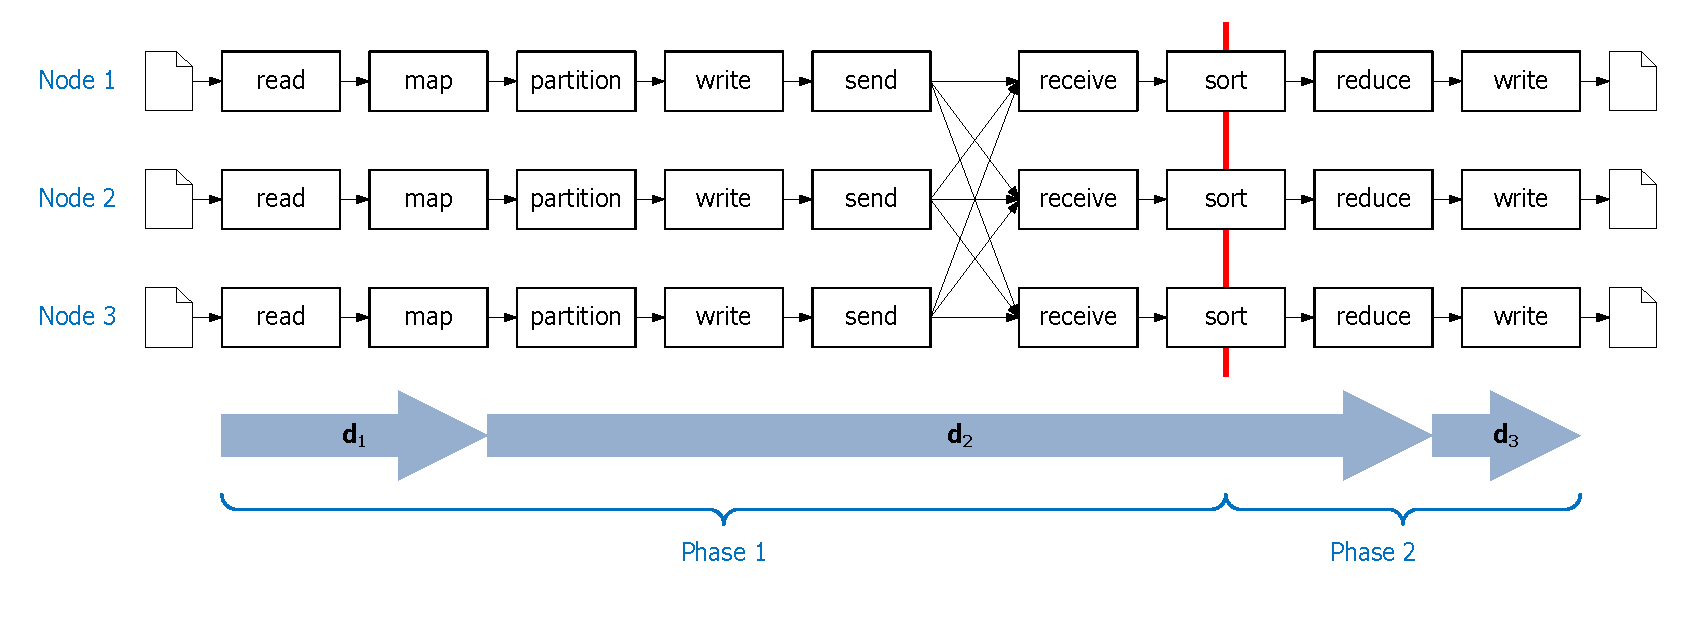
\epsfig{width=7in, angle=0, file=fig/mapreduce.ps}
\caption{A map-reduce dataflow.}
\label{fig:mapreduce}
\end{center}
\end{figure*}

Figure \ref{fig:mapreduce} illustrates the pipeline of an ideal map-reduce
computation involving three nodes. The computation is divided into two phases,
labeled Phase 1 and Phase 2, where each phase consists of operators that can
execute in parallel, as explained in the following section.

Figure \ref{fig:mapreduce} also illustrates how the amount of data ``flowing''
through the system changes throughout the computation. The amount of input data
per node is $d_1$, and the amount of output data per node is $d_3$. The amount
of data per node produced by the map operator and consumed by the reduce
operator is $d_2$. In most applications, the amount data flowing through the
system either remains the same or decreases (ie, $d_1 \ge d_2 \ge d_3$). For
example, in a distributed ``grep'' computation, $d_1 > d_2$ and $d_2 = d_3$. In
a distributed sort computation there is no data reduction, so $d_1 = d_2 =
d_3$.

\subsubsection{Phase 1}

Phase 1 begins with the reading of the input data from disk, and ends with the
sort operator. It includes the exchange of data over the network.

The first
write operator in Phase 1 is responsible for writing the output of the map
operator to persistent storage. Although this operator is not required in order to perform a map-reduce computation, it increases the system's ability to cope with hardware and software failures, as well as other
events that may cause a task to stop running (eg, a task might be killed by a
job-scheduling system to allow a higher-priority job to run on the same
cluster). Without this mechanism, if a single reduce task stops running, all of the map tasks must be re-executed. When running a long computation on a large cluster, where it is
likely that one of the tasks will stop running during the computation, it is a
good idea to include this step. However, if the total number of ``machine
hours'' required for a computation is small, the performance benefit from
omitting this step probably outweighs the cost of having to re-run the
computation if one of the tasks stops running during the original
computation.

In some map-reduce implementations, such as Google's MapReduce and Hadoop, the
output of the map operator is written to disk and then read back from disk
before sending the data over the network. This approach is inefficient because
it involves the unnecessary step of reading the entire data from disk.

It is also worth noting that parallel dataflow systems often
utilize underlying distributed file systems, such as GFS \cite{gfs}, in which a node's input data
may reside on a different node, but in most cases such systems are able to
schedule the execution tasks so that input data is read from the local disks
\cite{mapreduce}.

\subsubsection{Phase 2}

Phase 2 begins with the sort operator, and ends with the writing of the output
data to disk. In systems that utilize distributed file systems in which the
same data is replicated accross multiple nodes, the output data must be sent to
all the nodes that will store the data on their local disks. This is not shown
in Figure \ref{fig:mapreduce}, but we do account for it in our analytical
model (see Table \ref{table:model3}).

\subsection{Dataflow Parallelism}

In this section we discuss the two forms of parallelism that occur in a
parallel dataflow system: partitioned parallelism and pipelined parallelism. We
then explain why processing time (aka CPU time) can be ignored in the context
of typical data-parallel programs running on an efficient parallel dataflow
system.

DeWitt and Gray \cite{paralleldatabases} divide the potential parallelism in a
database system into partitioned parallism and pipelined parallelism. A
data-parallel program running on a parallel dataflow system is similar to a
relational query in a database in that it consists of operators applied to
streams of data. Partitioned parallelism is achieved by partitioning the data
and splitting an operator into multiple operators running on different
``processors.'' Pipelined parallelism, on the other hand, is achieved by
streaming the output of one operator into the input of another operator so that
the two operators can work in series.

Figure \ref{fig:mapreduce} outlines partitioned parallelism and pipelined
parallelism in an ideal map-reduce computation. Partitioned parallelism takes place on the
vertical axis. The input data is split between three nodes, and each operator
(eg, read, map) is, in fact, split into three sub-operators. Each of the three
sub-operators runs on a different node, thereby providing partitioned
parallelism. The primary focus of previous work on parallel dataflow systems
has been on providing large-scale partitioned parallelism.

Pipelined parallelism takes place on the horizontal axis of Figure
\ref{fig:mapreduce}. Specifically, the operators within each phase take
advantage of pipelined parallelism, but pipelined parallelism cannot occur
between operators in different phases.

Referring to the ideal map-reduce computation illustrated in Figure \ref{fig:mapreduce}, the read
operator is responsible for reading input data from disk. The data is read from
disk as a stream, so each record that is read from disk can be immediately
passed to the map operator, which can convert (ie, ``map'') that record into
zero or more records, which are then passed to the partition operator, and so
forth. In other words, the map operator does not need to wait for all of the
input to be read from disk, and the partition operator does not need to wait
for the map operator to finish operating on all of the records. The only
operator in Figure \ref{fig:mapreduce} that does not support pipelined
parallelism is the sort operator. The sort operator can only produce its first
output record after it has received all of its input records. (The last input
record might be the first in sorted order.)

The sort operator itself is actually a series of operators, so it is helpful to zoom into the details. There are two variants of the sort operator. One performs in-memory sorting, and is used if the data to be sorted fits in memory. The other performs an external (aka two-pass) sort, and is used if the data to be sorted does not fit in memory.

\begin{figure}
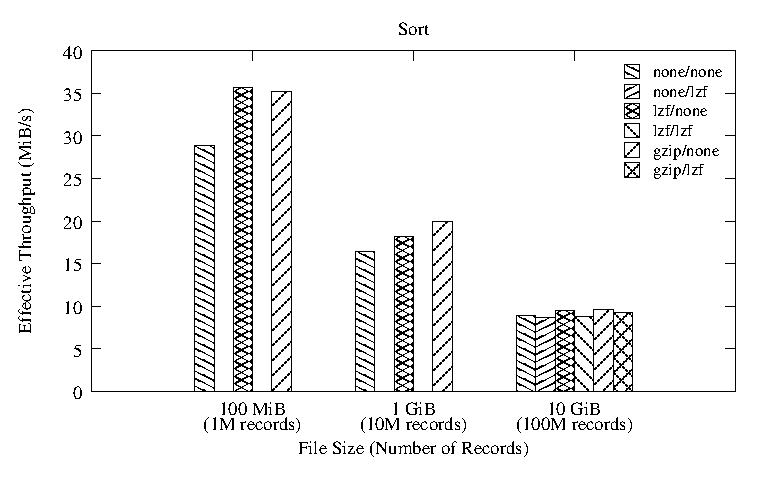
\epsfig{width=3.2in, angle=0, file=fig/sort.ps}
\caption{The sub-operators of the sort operator. Left: Our in-memory sort first arranges the records in buckets, then sorts the buckets individually and finally copies (ie, gathers) the records into contiguous blocks of memory. Right: An external sort involves sorting batches of records, writing each batch to disk, and finally merging the files to produce a sorted stream of records.}
\label{fig:sort}
\end{figure}

Our implementation of in-memory sorting in PDS includes three operators, as
shown on the left side of Figure \ref{fig:sort}:
\begin{itemize}
  \item Bucket: For each input record, place a pointer to the record in a bucket based on the first few bytes of the key field.
  \item Sort buckets: Sort each bucket using a standard quicksort algorithm.
  \item Gather: Iterate over all of the buckets and pointers in sorted order,
  and copy the actual records into contiguous memory.
\end{itemize}

Our in-memory sorting strategy, which consists of three operators, allows us to
pipeline most of the work with other operators in the overall map-reduce
computation. The bucket operator can be pipelined with Phase 1, and the gather
operator can be pipelined with Phase 2. The only actual operator that cannot be
pipelined with other operators is the sort buckets operator. However, this
operator offers the opportunity for partitioned parallelism within the node by
dividing the buckets among the node's CPU cores. With four cores, we were
able to sort 10 million 100-byte records, divided into $2^{16}$ buckets, in 0.3
seconds. That is, the sort buckets operator achieved a throughput of 33.33
million records per second, or 3.3 GB/s.

Our implementation of external sorting in PDS includes four operators, as
shown on the right side of Figure \ref{fig:sort}:
\begin{itemize}
  \item In-memory sort: Read as much data as fits into memory, and then
  sort it using the three operators of the in-memory sorting described earlier.
  \item Write: Write each memory-sized batch of data to a file on disk.
  \item Read: Read the sorted files from disk. The merge operator decides which
  file to read next, and how many records to read from it.
  \item Merge: Merge the records from the files into one long sorted stream.
\end{itemize}

One interesting aspect of the external sort is that it includes an operator
(in-memory sort) that is quite different from the typical streaming
operator. The in-memory sort, as described earlier, actually consists of three
operators and cannot offer full pipelined parallelism. However, in the context
of an external sort, in which the amount of data per node after the map
operation is significantly greater than the amount of memory available on a
node, we can actually achieve pipelined parallelism in the in-memory sort
operator (but at a courser granularity). For instance, if we consider the
stream of records flowing into the sort operator in Figure \ref{fig:mapreduce},
and we divide it into batches where the size of each batch is slightly less
than 50\% of the node's available memory, then the bucket operator can operate
on one batch while the gather operator is opereating on the previous batch.
There is some loss of pipelined parallelism in the first and last batches, but
if there is a sufficient amount of data to sort, then this loss is
insignificant.

\subsubsection{Computation}

Our efficiency model is designed to provide a tight lower bound on the
execution time of a data-parallel program. From the beginning, it was clear to
us that it would be difficult to account for computation in our model. Unlike
hard disks and network interfaces, where one can easily determine the sustained
throughput (in MB/s), it is much harder to reason about the ``throughput'' of a
CPU due to the plethora of architectures, the interaction with other components
of the system (eg, caches, memory) and the dependency on the program itself
(eg, branches, memory access locality).

We believe that there is a large class of problems for which the CPU-intensive operators operate at
throughputs that are significantly greater than that of the I/O intensive
operators. Fortunately, all of the CPU-intensive operators -- map, partition,
bucket, sort buckets, gather, reduce -- with the exception of sort buckets, take place in
pipelined parallelism with operators that read/write from/to disk and
send/receive to/from the network, so we can ignore the CPU-intensive operators
for such problems. Furthermore, the sort buckets operator,
which cannot be pipeline-parallelized with other operators, is so fast that it too can be
ignored.

As the number of CPU cores per node continues to increase in the upcoming
years, the class of problems for which the CPU-intensive operators are
significantly faster than the I/O-intensive operators will grow. Although there
will still be problems that do not fall into this category, we believe that
such problems will continue to be addressed by a different class of systems --
either job scheduling systems, for problems that are trivially parallelizable, or high-performance computing (HPC)
systems, for problems that require a large amount of inter-node communication.

\subsection{Optimal Execution Time}

Referring to Figure \ref{fig:mapreduce}, we can isolate all of the I/O
operations that must occur in each of the phases (depending on whether or not
an external sort is needed, of course). Table \ref{table:operations1} lists
these operations. Note that the fraction of $d_2$ that is sent
over the network is $\frac{n-1}{n}$, because each node ``sends'' $\frac{1}{n}$ of the data to itself.

\begin{table}
\centering
\begin{minipage}{0.5\textwidth}
\centering
\renewcommand{\arraystretch}{1.2}
\begin{tabular}{|l|l|l|}
\hline
        & $d_2 < \text{memory}$          & $d_2 \gg \text{memory}$ \\ \hline
Phase 1 & Disk read:  $d_1$              & Disk read:  $d_1$ \\ 
        & Disk write\footnote{This ``backup write'' is optional.}: $d_2$ & Disk write: $d_2$ \\
        & Network: $\frac{n-1}{n} d_2$   & Network: $\frac{n-1}{n} d_2$ \\
        &                                & Disk write: $d_2$ \\ \hline
Phase 2 & Disk write: $d_3$              & Disk read: $d_2$ \\
        &                                & Disk write: $d_3$ \\ \hline
\end{tabular}
\caption{The I/O-operations in a map-reduce parallel dataflow system.}
\label{table:operations1}
\end{minipage}
\end{table}

Many parallel dataflow systems utilize distributed file systems, such as GFS \cite{gfs} and HDFS \cite{hdfs}. Such file systems typically use replication and store multiple copies of each block of data. In most cases, the tasks of a data-parallel program can be scheduled so that the input data is read locally and does not need to be sent over the network. However, at the end of the last phase, each node must send its output data to $r - 1$ other nodes, where $r$ is the file system's replication factor. The sending node, along with the $r - 1$ receiving nodes, write the data to their their local disks, thereby ensuring that $r$ copies of the data are stored. Obviously, all of these operations occur in parallel to the other operations of the last phase of the computation. Table \ref{table:operations2} lists the I/O-related operations that take place in a parallel dataflow system that utilizes a distributed file system with $r$-way replication.

\begin{table}
\centering
\begin{minipage}{0.5\textwidth}
\centering
\renewcommand{\arraystretch}{1.2}
\begin{tabular}{|l|l|l|}
\hline
        & $d_2 < \text{memory}$           & $d_2 \gg \text{memory}$ \\ \hline
Phase 1 & Disk read: $d_1$                & Disk read: $d_1$ \\ 
        & Disk write\footnote{This ``backup write'' is optional.}: $d_2$ & Disk write: $d_2$ \\
        & Network: $\frac{n-1}{n} d_2$    & Network: $\frac{n-1}{n} d_2$ \\
        &                                 & Disk write: $d_2$ \\ \hline
Phase 2 & Network: $\left(r-1\right) d_3$ & Disk read: $d_2$ \\
        & disk write: $r d_3$             & Network: $\left(r-1\right) d_3$ \\
        &                                 & Disk write: $r d_3$ \\
        \hline
\end{tabular}
\caption{The I/O-operations in a map-reduce parallel dataflow system that utilizes a distributed file system with $r$-way replication.}
\label{table:operations2}
\end{minipage}
\end{table}

Following our conclusion that for many data-parallel progrems, only
I/O-intensive operators have a real impact on the execution time the program,
we can easily determine the execution time based on Tables
\ref{table:operations1} and \ref{table:operations2}.

\begin{table}
\centering
\begin{minipage}{0.5\textwidth}
\centering
\renewcommand{\arraystretch}{1.2}
\begin{tabular}{|l|p{6.5cm}|}
\hline
Symbol & Definition \\ \hline
$n$    & The number of nodes in the cluster. \\ \hline
$D$    & The aggregate disk throughput of a single node. For example,
a node with four disks, where each disk provides 65 MB/s, would have $D$ = 260
MB/s.\footnote{In reality, $D$ depends on the actual file system, and on
how the blocks are placed on the disks' tracks. An application cannot obtain
the highest throughput offered by the raw disk devices. Therefore, if possible,
it is preferrable to obtain the value of $D$ empirically.} \\ \hline
$N$    & The network throughput of a single node. After accounting for unavoidable overhead, gigabit Ethernet provides roughly $N$ = 110 MB/s. \\ \hline
$r$    & The replication factor of the distributed file system. If a
distributed file system is not used, or no replication is used, $r$ = 1. \\
\hline
$i$    & The total amount of input data for a given computation. \\ \hline
$d_1$  & The amount of input data per node, for a given computation. ($d_1 =
\frac{i}{n}$) \\ \hline
$d_2$  & The amount of data per node after the map operator, for a given
computation. ($d_2 = \frac{i \cdot e_M}{n}$) \\ \hline
$d_3$  & The amount of output data per node, for a given computation. ($d_3 =
\frac{i \cdot e_M \cdot e_R}{n}$) \\ \hline
$e_M$  & The ratio between the map operator's output and its input. ($e_M =
\frac{d_2}{d_1}$) \\ \hline $e_R$  & The ratio between the
reduce operator's output and its input. ($e_R = \frac{d_3}{d_2}$) \\ \hline

\end{tabular}
\caption{The parameters that describe the hardware configuration of a parallel dataflow system and the workload running on it.}
\label{table:symbols}
\end{minipage}
\end{table}

Table \ref{table:model1} shows the execution time of a computation on a
parallel dataflow system for four different scenarios. (The symbols are defined
in Table \ref{table:symbols}.) We assume that the parallel dataflow system is
being used only for a single data-parallel program. Although this is typically
not the case in real-world deployments, it simplifies the model and allows us
to relate the performance of other systems, such as Google's MapReduce and
Dryad, to our model. We further assume that the system either does not
use a distributed file system, or that it does not use replication. (This
assumption is relaxed later.)

\begin{table*}
\centering
\renewcommand{\arraystretch}{1.2}
\begin{tabular}{|l|l|l|}
\hline
& $d_2 < \text{memory}$ & $d_2 \gg \text{memory}$ \\ \hline
Without backup write & $max\left\{\frac{d_1}{D},
\frac{\frac{n-1}{n} d_2}{N}\right\} + \frac{d_3}{D}$ & $max\left\{\frac{d_1 +
d_2}{D}, \frac{\frac{n-1}{n} d_2}{N}\right\} + \frac{d_2 + d_3}{D}$ \\ \hline
With backup write & $max\left\{\frac{d_1 + d_2}{D}, \frac{\frac{n-1}{n} d_2}{N}\right\} +
\frac{d_3}{D}$ & $max\left\{\frac{d_1 + 2 d_2}{D},
\frac{\frac{n-1}{n} d_2}{N}\right\} + \frac{d_2 + d_3}{D}$ \\ \hline
\end{tabular}
\caption{The execution time of a map-reduce computation on a parallel dataflow system. $D$ and $N$ are the disk and network throughputs of a single node, respectively.}
\label{table:model1}
\end{table*}

Since $d_1$, $d_2$ and $d_3$ depend on $n$, the number of nodes in the cluster, it is helpful to express the model as a function of $n$. Furthermore, it is usually easy for a developer to estimate  the extent of data reduction (or expansion) that the map and reduce operators of a given program achieve. Table \ref{table:model2} presents our model as a function of $i$, $n$, $e_M$ and $e_R$.

\begin{table*}
\centering
\renewcommand{\arraystretch}{1.2}
\begin{tabular}{|l|l|l|}
\hline
& $\frac{i \cdot e_M}{n}< \text{memory}$ & $\frac{i \cdot e_M}{n} \gg \text{memory}$ \\ \hline
Without backup write & $\frac{i}{n} \left( max\left\{\frac{1}{D},
\frac{\frac{n-1}{n} e_M}{N}\right\} + \frac{e_M e_R}{D} \right)$ & $\frac{i}{n}
\left( max\left\{\frac{1 + e_M}{D}, \frac{\frac{n-1}{n} e_M}{N}\right\} +
\frac{e_M + e_M e_R}{D} \right)$ \\ \hline With backup write & $\frac{i}{n}
\left( max\left\{\frac{1 + e_M}{D}, \frac{\frac{n-1}{n} e_M}{N}\right\} +
\frac{e_M e_R}{D} \right)$ & $\frac{i}{n} \left( max\left\{\frac{1 + 2 e_M}{D},
\frac{\frac{n-1}{n} e_M}{N}\right\} + \frac{e_M + e_M e_R}{D} \right)$ \\ \hline
\end{tabular}
\caption{The execution time of a map-reduce computation on a parallel dataflow system, as a function of the total amount of input data ($i$), and the map-reduce data expansion ratios ($e_M$ and $e_R$).}
\label{table:model2}
\end{table*}

Table \ref{table:model3} is an extention of Table \ref{table:model2} that
accounts for distributed file systems with $r$-way replication. Note that $r$
is the actual replication factor used for the computation's output file, which
may be different from the file system's default replication factor.

\begin{table*}
\centering
\renewcommand{\arraystretch}{1.2}
\begin{tabular}{|l|l|l|}
\hline
& $\frac{i \cdot e_M}{n}< \text{memory}$ \\ \hline
Without backup write &
$\frac{i}{n} \left( max\left\{\frac{1}{D}, \frac{\frac{n-1}{n} e_M}{N}\right\} +
max\left\{\frac{r e_M e_R}{D}, \frac{e_M e_R \left(r - 1\right)}{N}\right\} \right)$ \\ \hline
With backup write & $\frac{i}{n} \left( max\left\{\frac{1 + e_M}{D},
\frac{\frac{n-1}{n} e_M}{N}\right\} + max\left\{\frac{r e_M e_R}{D}, \frac{e_M
e_R \left(r - 1\right)}{N}\right\} \right)$ \\ \hline

& $\frac{i \cdot e_M}{n} \gg \text{memory}$ \\ \hline
Without backup write & $\frac{i}{n} \left( max\left\{\frac{1 + e_M}{D},
\frac{\frac{n-1}{n} e_M}{N}\right\} + max\left\{\frac{e_M + r e_M e_R}{D},
\frac{e_M e_R \left(r - 1\right)}{N}\right\} \right)$ \\ \hline
Without backup write & $\frac{i}{n} \left(
max\left\{\frac{1 + 2 e_M}{D}, \frac{\frac{n-1}{n} e_M}{N}\right\} +
max\left\{\frac{e_M + r e_M e_R}{D}, \frac{e_M e_R \left(r -
1\right)}{N}\right\} \right)$ \\ \hline

\end{tabular}
\caption{The execution time of a map-reduce computation on a parallel dataflow system in which output data is replicated accross $r$ nodes.}
\label{table:model3}
\end{table*}

\subsection{Common Workloads: Grep and Sort}

In this section we apply our efficiency model to two computations. The grep
computation searches through data looking for a particular pattern, while the
sort computation sorts data. According to \cite{mapreduce}, these two programs
are representative of a large subset of the real programs written by users of
Google's MapReduce -- one class of programs extracts a small amount of
interesting data from a large data set, and another class shuffles data from
one representation to another.

For a distributed grep computation that ``selects'' only a small portion of the input data, $e_M \approx 0$ and $e_R = 1$ (so $e_M e_R \approx 0$). For distributed sort, $e_M = e_R = 1$. Referring to Table \ref{table:model2}, the execution time of a distributed grep computation is:
\begin{equation}
t_\text{grep} = \frac{i}{n D}
\label{eqn:grepmodel}
\end{equation}
This result is not surprising, because in a highly selective grep computation
the map operator significantly reduces the amount of data, so only a negligible
amount is written to the backup files, sent over the network and written to the output
files.

The execution time for a sort computation depends on which of the four
scenarios in the model (Table \ref{table:model2} or \ref{table:model3})
applies. For example, if a backup write is used, and the input data is sufficiently large to require an
external sort, then we refer to the bottom-right corner of Table
\ref{table:model2}:
\begin{equation}
t_\text{sort} = \frac{i}{n} \left( max\left\{\frac{3}{D}, \frac{n-1}{n
N}\right\} + \frac{2}{D} \right)
\label{eqn:sortmodel1}
\end{equation}
As another example, if the amount of data per node is small, the data can be sorted in memory, and the computation will likely be too short to warrant the use of backup files. In this case, we refer to the top-left corner of Table \ref{table:model2}:
\begin{equation}
t_\text{sort} = \frac{i}{n} \left( max\left\{\frac{1}{D}, \frac{n-1}{n
N}\right\} + \frac{1}{D} \right)
\label{eqn:sortmodel2}
\end{equation}

\subsection{Insights from the model}

\subsubsection{Balancing disk and network}

When running a data-parallel program on more than one node, both disk and
network resources are consumed. In an efficient system, one of these two
resources will be fully utilized. Depending on the hardware configuration, the
other resource could be highly underutilized. In such cases, it is usually
possible to achieve higher ``throughput per dollar'' by creating a more balaned
system. For example, if the network is fully utilized, whereas the disks are
not, then it would probably make sense to reduce the number of disks per node.
Alternatively, it may be beneficial to increase the network throughput by
replacing, for instance, the gigabit Ethernet network with a 10-gigabit Ethernet or Infiniband network.

Our model can assist in achieving a more balanced
hardware configuration. The $max\left\{\ldots\right\}$ components of the
formulas in Tables \ref{table:model1}, \ref{table:model2} and
\ref{table:model3} represent the tension between disk and network resources. In
a balanced system, the expressions within the $max\left\{\ldots\right\}$
components are equal.

\subsubsection{Investing in fault tolerance}

One of the widely publicized benefits of map-reduce frameworks, such as Hadoop,
is their ability to cope with failures (software and hardware) in the middle of
a computation. This capability is achieved via what we refer to as a ``backup
write,'' and is reflected in our model. In some scenarios, however, this level
of fault tolerance results in unnecessary overhead. For example, if we consider
a map-reduce computation with an in-memory sort, as shown on the left side of
Table \ref{table:model2}, we can identify three possible situations:

\begin{itemize}
  \item $\frac{\frac{n-1}{n} e_M}{N} \ge \frac{1+e_M}{D}$: The backup write does
  not cost anything, because the throughput is limited by the network.
  \item $\frac{1}{D} < \frac{\frac{n-1}{n} e_M}{N} < \frac{1+e_M}{D}$: The
  backup write reduces the throughput, causing it to be limited by disk rather than network.
  \item $\frac{\frac{n-1}{n} e_M}{N} \le \frac{1}{D}$: The backup write reduces
  the throughput, and disk remains the limiting factor.
\end{itemize}

In the first case, it is clearly beneficial to perform a backup write, because
it is ``free'' (due to pipelined parallelism). In the other cases, however, we
must first predict the probability of a failure, and then the expected number
of times that the entire computation would need to be restarted, in order to
decide whether a backup write is worthwhile.

Referring to Table \ref{table:model2}, if an in-memory sort is feasible, the
total number of node-seconds is:

\begin{equation*}
t = i \left( max\left\{\frac{1}{D},
\frac{\frac{n-1}{n} e_M}{N}\right\} + \frac{e_M e_R}{D} \right)
\end{equation*}

If we denote $p$ as the probability that a single node will fail (or stop
running, for any other reason) while running for a period of length $t$, then
the expected execution time of a computation that does not use backup
writes (and thus has to execute again with probability $p$) is roughly:

\begin{equation}
\frac{i}{n \cdot p} \left( max\left\{\frac{1}{D},
\frac{\frac{n-1}{n} e_M}{N}\right\} + \frac{e_M e_R}{D} \right)
\label{eqn:timewithoutbackup}
\end{equation}

We can then compare this to the execution time of a computation that does use
backup writes:

\begin{equation}
\frac{i}{n} \left( max\left\{\frac{1+e_M}{D},
\frac{\frac{n-1}{n} e_M}{N}\right\} + \frac{e_M e_R}{D} \right)
\label{eqn:timewithbackup}
\end{equation}

If the value of Equation \ref{eqn:timewithbackup} is less than the value of
Equation \ref{eqn:timewithoutbackup} then the expected execution time when
using backup writes is less than the expected execution time when not using
backup writes, and vice versa.

\subsubsection{The data exchange wall}

The data exchange wall is a phenomenon where the aggregate throughput of a
data-parallel program running on $n$ nodes is less than the throughput of the
same program running on a single node. It is easy to see why this might happen
in an efficient parallel dataflow system that performs similarly to our model.
For example, referring to the execution time of a distributed sort shown in
Equation \ref{eqn:sortmodel2}, if $\frac{n}{n-1} N < D$, then the aggregate
throughput of the sort computation is: \[T_\text{sort} = \frac{i}{t} =
\frac{n}{\frac{n-1}{n N} + \frac{1}{D}}\] When running on a single node:
\[T_\text{sort} = \frac{i}{t} = \frac{n}{\frac{1}{D} + \frac{1}{D}} =
\frac{D}{2}\] In this specific example, if $D > 6 N$, then the aggregate
throughput on \emph{two} nodes will be lower than the throughput of a single
node. Considering the recently published hardware configuration at Google
\cite{sorting1pb}, in which each node has 12 disks and the nodes are connected
via gigabit Ethernet, and estimating that the throughput of a single disk is 65
MB/s, we have: $D = 12 \cdot 65 \text{ MB/s} = 780 \text{ MB/s}$ and $N = 110
\text{ MB/s}$.

\section{Efficiency Evaluation of Existing Systems}

In this section we evaluate the performance of various parallel dataflow
systems with respect to our model. We compare the actual throughput with the
optimal throughput, and also examine how much hardware would be needed
to obtain the reported throughput given an optimal system. Since all of the
experiments in this section involved at least 1000 nodes, we can safely ignore
the $\frac{n-1}{n}$ factor in the formulas. Also, all of these experiments
were executed on idle clusters (ie, clusters that were not running any other
jobs at the same time), so there is no need to consider potential interferences
from other jobs.

\subsection{Hadoop -- TeraSort}

Hadoop currently holds the record \cite{hadoop2009} for sorting 1 TB of data in
the Sort Benchmark \cite{sortbenchmark} format. The following symbols describe
the experiment: $i = 1 \text{ TB}$, $n = 1460$, $D = 4 \cdot 65 = 260 \text{ MB/s}$, $N = 110 \text{ MB/s}$, $d_2 = i/n = 685 \text{ MB}$.

With only 685 MB per node, the data can be sorted by the individual nodes in memory. A backup write is not beneficial, in this case, so we can apply Equation \ref{eqn:sortmodel2} to obtain the optimal execution time:
\[t_\text{optimal} = \frac{1000000}{1460} \left( \frac{1}{110} + \frac{1}{260}
\right) = 8.86 \text{ seconds}\]
After fine-tuning the system for this specific
benchmark, Yahoo achieved $t_\text{actual} = 62$ seconds -- over six times
slower than the optimal performance. Furthermore, an optimal system using
the same node hardware would be able to achieve the same throughput as Hadoop
with about 270 nodes instead of 1460. (Note that it is possible to achieve full
backplane bandiwdth for 270 nodes.)

\subsection{MapReduce -- TeraSort}

Google recently ran \cite{sorting1pb} the TeraSort benchmark on 1000 nodes with
12 disks in each node. The following symbols describe the experiment: $i = 1 \text{ TB}$, $n = 1000$, $D = 12 \cdot 65 = 780 \text{
MB/s}$, $N = 110 \text{ MB/s}$, $d_2 = i/n = 1000 \text{ MB}$.

As with Yahoo's TeraSort experiment (with Hadoop), we can apply Equation \ref{eqn:sortmodel2} to obtain the optimal execution time:
\[t_\text{optimal} = \frac{1000000}{1000} \left( \frac{1}{110} + \frac{1}{780}
\right) = 10.37 \text{ seconds}\]
Google achieved $t_\text{actual} = 68$
seconds -- over six times slower than the optimal performance. Furthermore, an
optimal system using
the same node hardware would be able to achieve the same throughput as Google's
MapReduce with about 170 nodes instead of 1000. (Note that it is possible to achieve full
backplane bandiwdth for 170 nodes.)

\subsection{Hadoop -- PetaSort}
Although similar in nature to their TeraSort experiment, Yahoo's PetaSort experiment with Hadoop introduces several differences:
\begin{itemize}
  \item Due to the larger amount of data, the computation is much longer, so
  using a backup write is justified.
  \item There were $n = 3658$ nodes, so there was far more data per node ($d_2 = 273.37 \text{ GB}$) than can be fit into memory. Therefore, an external sort is necessary.
  \item The output of the computation was stored on HDFS with two-way replication, so we must use Table \ref{table:model3} rather than Table \ref{table:model2}.
\end{itemize}

The following symbols describe
the experiment: $i = 1 \text{ PB}$, $n = 3658$, $D = 4 \cdot 65 = 260 \text{
MB/s}$, $N = 110 \text{ MB/s}$, $d_2 = i/n = 273.37 \text{ GB}$.

Referring to the bottom cell of Table \ref{table:model3}:
\begin{align*}
t_\text{optimal} &= \frac{i}{n} \left( max\left\{\frac{3}{D}, \frac{1}{N}\right\} + max\left\{\frac{3}{D}, \frac{1}{N}\right\} \right)\\
  &= \frac{1000000000}{3658} \left( max\left\{\frac{3}{260}, \frac{1}{110}\right\} + max\left\{\frac{3}{260}, \frac{1}{110}\right\} \right)\\
  &= 6308.61 \text{ seconds}
\end{align*}
Yahoo achieved $t_\text{actual} = 58500$ seconds -- about 9.27 times slower
than the optimal performance. Furthermore, an
optimal system using the same node hardware would be able to
achieve the same throughput as Hadoop with less than 400
nodes instead of 3658.

Since Yahoo's cluster consisted of a large number of nodes, it is worth
considering the issue of backplane bandwidth. Although it is difficult
to construct a network that can provide full bisection bandwidth for 3658 nodes
(with gigabit Ethernet interfaces), it is certainly possible to do so for 400
nodes (by using high-end switches).

Re-visiting Yahoo's result, the average throughput per node was
$\frac{1000000000/3658 MB}{58500 s} = 4.67 MB/s$. Since two-way replication was
used, each fragment of data was sent over the network twice: once for
the data exchange, and once for storing the second replica on the distributed file
system. Yahoo used one switch and 40 nodes per rack, and connected the rack
switches to the core switch via 8 gigabit Ethernet connections. That is, each
rack switch had an 8 Gb/s connection to the core switch (in each direction). The
vast majority of the network traffic ($90/91$) was between racks, so the actual
throughput achieved on these uplinks was only $90/91 \cdot 40 \cdot 4.67 =
184.87 MB/s$ MB/s in each direction.

\subsection{MapReduce -- PetaSort}

Although similar in nature to their TeraSort experiment, Google's PetaSort
experiment introduces several differences:
\begin{itemize}
  \item Due to the larger amount of data, the computation is much longer, so
  using a backup write is important. In fact, Google ran the experiment
  multiple times, and at least one disk broke during each execution.
  \item There were $n = 4000$ nodes, so there was far more data per node ($d_2
  = 250 \text{ GB}$) than can be fit into memory. Therefore, an external sort
  is necessary.
  \item The output of the computation was stored on GFS with three-way
  replication, so we must use Table \ref{table:model3} rather than Table
  \ref{table:model2}.
\end{itemize}

The following symbols describe
the experiment: $i = 1 \text{ PB}$, $n = 4000$, $D = 12 \cdot 65 = 780 \text{ MB/s}$, $N = 110
\text{ MB/s}$, $d_2 = i/n = 250 \text{ GB}$. 

Referring to the bottom cell of Table \ref{table:model3}:
\begin{align*}
t_\text{optimal}
  &= \frac{i}{n} \left( max\left\{\frac{3}{D},
\frac{1}{N}\right\} + max\left\{\frac{4}{D}, \frac{2}{N}\right\} \right)\\ 
  &= \frac{1000000000}{4000} \left( max\left\{\frac{3}{780},
 \frac{1}{110}\right\} + max\left\{\frac{4}{780}, \frac{2}{110}\right\}
 \right)\\ &= 6818 \text{ seconds} 
\end{align*}
Google achieved $t_\text{actual} = 21720$ seconds -- about 3.2 times slower than
the optimal performance. Furthermore, an optimal system using
the same node hardware would be able to
achieve the same throughput as Google's MapReduce with about 1250 nodes instead
of 4000. Also, according to our model, for the purpose of map-reduce
computations, Google's nodes are over-provisioned with disks. In an optimal
system, the network would be the bottleneck even if each node had only 6
disks instead of 12.

Google did not describe the network topology used in their experiment, so we
cannot account for any limitations on backplane bandwidth. However, the fact
that MapReduce was 3.2 times slower than the optimal performance
indicates that some resources were significantly underutilized. For example, if
the bottleneck was the network's backplane bandwidth, then Google should have
been able to achieve the same performance with 3.2 times less nodes per switch
(and, overall 3.2 times less nodes).

\subsection{MapReduce -- Grep}

The original MapReduce paper \cite{mapreduce} described a distributed grep
computation that was executed on MapReduce. The following symbols describe
the experiment: $i = 1 \text{ TB}$, $n = 1800$, $D = 2 \cdot 50 = 100 \text{ MB/s}$, $N = 110
\text{ MB/s}$, $d_2 = 9.23 \text{ MB}$, $e_M = 9.23/1000000 \approx 0$, $e_R =
1$.

Note that the paper does not specify the throughput of the disks. Therefore, we
looked at the specifications of disks from the same time (2003-2004), and
estimate that a single disk provided a throughput of 50 MB/s. According to
Equation \ref{eqn:grepmodel}, the optimal execution time for these parameters
is:
\[t_\text{optimal} = \frac{i}{n D} = 5.56 \text{ seconds}\]
Google achieved $t_\text{actual} = 150$ seconds including startup overhead, or
90 seconds without that overhead -- still about 16.19 times slower than the
optimal throughput. Furthermore, an optimal system using
the same node hardware would be able to achieve the
same throughput as Google's MapReduce with less than 70 nodes instead of 1800!

\subsection{Dryad}

Although our model is built around the map-reduce programming model, it can be
applied it to other systems with similar characteristics. For example,
Microsoft's data mining experiment on Dryad \cite{dryad} involved very high
selectivity ($e_M = 0.015$) during its first phase. Since the remaining phases
were not CPU-intensive, their execution time should be insignificant compared to
the execution time of the first phase. Therefore, we can use Equation
\ref{eqn:grepmodel}. The following symbols describe
the experiment: $i = 10160519 \text{ MB}$, $n = 1800$, $D = 4 \cdot 65 = 260
\text{ MB/s}$, $N = 110 \text{ MB/s}$, $d_2 \approx 0$. \[t_\text{optimal} = \frac{i}{n D} =
21.71 \text{ seconds}\]

Microsoft achived $t_\text{actual} = 690$ seconds -- 31.78 times slower than
the optimal. It is worth noting that our optimal time is not accurate, because
we ignored all but the first of the four steps in the computation (see Figure
10 in the Dryad paper \cite{dryad}). However, since the first step involved
10.2 TB of data, and the other steps involve only 154 GB, 118 GB and 33.4 GB,
and none of the steps seem to be CPU-bound, the first step is expected to
consume the vast majority of execution time and resources.

\section{Parallel DataSeries}

DataSeries \cite{dataseries} is an on-disk data format and open-source run-time
library that is optimized for analyzing structured serial data (a series of
records that share a common structure). DataSeries files are stored as
sequences of \emph{extents}, where each extent is a series of records.
The data is read and processed at the granularity of extents, and a DataSeries
module is a C++ class that implements a single virtual function ($\tt
getExtent$) that returns an extent (or $\tt NULL$, if no more extents
are available).

The DataSeries run-time library makes it easy to develop C++ applications that
read, process and write DataSeries files. A typical application utilizes existing
DataSeries modules (eg, a $\tt SourceModule$ that retrieves extents from a
DataSeries file), as well as application-specific modules. The modules are
typically organized in a pipeline, so that each module invokes its upstream
module's $\tt getExtent$ function to obtain data. In addition to modules,
DataSeries provides a component named $\tt DataSeriesSink$, which consumes
extents from an upstream module and writes them to a DataSeries file. The
pipeline of an application that reads a DataSeries file, processes it and then
writes a new DataSeries file, is structured as: $\tt SourceModule$ $\to$
\emph{one or more filter modules} $\to$ $\tt DataSeriesSink$. Although $\tt DataSeriesSink$
is an integral part of a DataSeries pipeline, it is not technically a module,
because it does not implement the module interface ($\tt getExtent$).

We developed Parallel DataSeries (PDS), an extension of DataSeries that enables
develelopers to create and execute DataSeries-based programs on multiple cores
(intra-node parallelism) and multiple nodes (inter-node parallelism).

\subsubsection{Itra-node parallelism}

Achieving intra-node parallelism involved exploiting both pipelined parallelism
and partitioned parallelism in the context of a single node. To achieve
pipelined parallelism on a single node (with multiple cores), we developed a
module named $\tt PrefetchBufferModule$, which calls its upstream module's $\tt
getExtent$ function within a dedicated thread. $\tt PrefetchBufferModule$
includes a small buffer that stores a limited number of extents, retrieved from its upstream module, until those extents are requested by its downstream
module. A developer can use a $\tt
PrefetchBufferModule$ module to split the pipeline on a node so that the
modules that are upstream from the $\tt
PrefetchBufferModule$ module can run in parallel to the modules that are
downstream from the module. A pipeline can, of course, include more than one
$\tt PrefetchBufferModule$ module (ie, one such module can be integrated
between every two modules).

Achieving partitioned parallelism on a single node requires the invidividual
modules to be ``smart'' about how they process the data that they receive from
their upstream modules. For some modules, such as the sorting module that we
developed ($\tt SortModule$), the best approach is to build the
parallelism into the module. For many other modules, where parallelism is more
``natural,'' we developed an abstract class, $\tt ParallelFilterModule$.
Developers of such modules can inherit from $\tt ParallelFilterModule$ and
implement a single function, $\tt createNextExtent$, which should obtain the
next extent from the upstream module, process it and return the resulting
extent. We used this technique to implement $\tt GrepModule$.

\subsubsection{Inter-node parallelism}

After considering many potential architectures for supporting inter-node
parallelism, we realized that the most natural design would be to implement a
single module: $\tt NetworkModule$. Like any other DataSeries filter module, it is initialized with an upstream module, from which
it pulls extents via the $\tt getExtent$ function. In addition, $\tt
NetworkModule$ receives three additional parameters:
\begin{itemize}
  \item A list of all the nodes that will take part in the computation.
  \item The index of the current node within the list of nodes.
  \item A partitioner object, which determines the partition for each
  record. That is, $\tt NetworkModule$ asks the partitioner which partition a
  given record belongs to.
\end{itemize}

Each node participating in a computation is responsible for a single
partition, so in a computation involving 10 nodes, each of the nodes'
$\tt NetworkModule$ modules sends records belonging to partition 3 to node 3.
The unit of transmission is an extent, so $\tt NetworkModule$ collects many
records belonging to the same partition into an extent, and sends the extent once it is
full. This is necessary because DataSeries pipelines operate on extents.

The $\tt NetworkModule$ module receives extents from other nodes over the
nework and hands them to the downstream module when its $\tt getExtent$ function is called. The
following is a listing of a PDS-based grep program that sorts the matching
records.
\begin{mylisting}
\begin{verbatim}
string field_name("line");
string needle("abc"); // The pattern to search for.

SourceModule source_module(input_file_name, ...);
GrepModule<Variable32Field, Variable32FieldMatcher>
   grep_module(source_module, field_name,
               Variable32FieldMatcher(needle));

NetworkModule<Variable32Field, Variable32FieldPartitioner>
   network_module(grep_module, node_names, node_index,
                  field_name, Variable32FieldPartitioner());

SortModule<Variable32Field, Variable32FieldComparator>
   sort_module(network_module, field_name,
               Variable32FieldComparator());

DataSeriesSink sink(output_file_name, Extent::compress_none);
Extent *extent = NULL;
while ((extent = sort_module.getExtent()) != NULL) {
    sink.writeExtent(extent);
    delete extent;
}
\end{verbatim}
\end{mylisting}

It is worth noting that PDS does not currently utilize a distributed file
system, so the input files must be statically partitioned and placed on the nodes of the cluster.

\subsection{Engineering for Efficiency}

Our initial goal in building PDS was to understand whether it is possible to
build a parallel dataflow system that can fully utilize the underlying I/O
hardware.

As described earlier, a DataSeries-based program is essentially a pipeline of
modules, in which each module takes the output of an upstream module as its
input. While developing PDS, we tested each module seperately to make sure it
was operating at maximum speed.

\subsubsection{GrepModule}

After completing the first version of our grep
  module, we created a simple PDS program consisting of only two modules: $\tt
  SourceModule$ and $\tt GrepModule$. This program did not produce any output.
  Since we wanted to test $\tt GrepModule$, we ran the program several times,
  ensuring that the input file was cached by the OS. Since the $\tt
  SourceModule$ module itself was capable of achieving well over 1 GB/s on a
  cached file, this experiment allowed us to observe the actual throughput of
  $\tt GrepModule$. After several optimizations, including the replacement of
  our string matching algorithm (we ended up using Boyer-Moore-Horspool, a
  variant of Boyer-Moore \cite{boyermoore}), and better utilization of multiple
  cores, we were able to increase our throughput significantly.
  
\subsubsection{SortModule}

This module was far more challenging than $\tt
  GrepModule$, but we were able to use the same technique to test it in
  isolation. We first focused on developing an in-memory sort module ($\tt
  MemorySortModule$), and we then developed the more generic $\tt SortModule$
  that supported external (aka two-pass) sorting. We used $\tt MemorySortModule$
  to implement $\tt SortModule$, so once we were done optimizing $\tt
  MemorySortModule$, we could trust it as a ``black box'' while developing and
  optimizing $\tt SortModule$.
  
\subsubsection{NetworkModule}
  
This module can be tested without any ``real''  
  input data, so we developed $\tt NullModule$, a source module that produces
  extents at maximum speed. $\tt NullModule$'s $\tt getExtent$ method simply allocates  
  a block of memory for each new extent, without initializing it. We created a  
  PDS program that included just a $\tt NullModule$ module and a $\tt  
  NetworkModule$ module.
  
  Our initial implementation of $\tt NetworkModule$ was  
  unable to achieve full gigabit Ethernet throughput between all nodes. To
  understand the why this was happening, we utilized a number of microbenchmarks
  using both publicly available tools, such as $\tt netcat$, and our own simple benchm
 arks. For example, to discover the maximum ``all-to-all'' network throughput on our
 10-node cluster, we wrote a shell script that, when executed on each node, establishes
 a TCP connection with every other node and then sends an infinite stream
of data (from $\tt /dev/zero$) over each connection. For each TCP connection, we
used $\tt netcat$ (with the $-l$ flag on one of the sides) to transmit the data
over the network.
   
 Using these benchmarks, we were able to understand what was limiting the
 network throughput. First, our original implementation used only a single
 thread to send extents over the network. As a result, when the number of nodes increased, that thread would occasionally block while sending data to one of the other nodes (because the other node could be busy accepting an extent from a different node). We were able to overcome this problem by using a seperate sender thread for each node. (An alternative solution would be to use
  an event interface, such as epoll, or asynchronous IO.) Second, our original
  implementation established a seperate TCP connection in each direction, so
  each pair of nodes communicated over two TCP connections. This resulted in
  unnecessary contention due to the acknowledgement packets, so we improved the
  module by establishing only a single TCP connection between each pair of
  ndoes. Finally, we increased the Ethernet MTU to 8192 bytes (from 1500). These changes enabled us to achieve a full gigagbit Ethernet throughput between the nodes
  (about 110 MB/s in each direction).


\section{Efficiency Evaluation of PDS}

%% ProCurve Switch 2900-48G 

In this section we present our evaluation of PDS. We designed and executed
several experiments with the overall goal of understanding whether an actual
parallel dataflow system can achieve performance that is close to the optimal
performance outlined by our model.

We decided to experiment with distributed grep and sort computations, based on
Google's observation that these are representative of most of their MapReduce
jobs, as well as our own experience. Furthermore, although we are primarily
interested in comparing the performance of PDS to that of our theoretical
model, choosing grep and sort allows us to compare our results with other
systems that have been measured under these workloads.

\subsection{Grep}

We implemented a PDS program that that searches for a given substring in
a large, distributed file. Although unnecessary for an actual grep
implementation, we sorted the matching lines in order to provide the exact same
functionality as the grep experiments performed by Google \cite{mapreduce}. We
implemented our grep program by hooking up the following modules:
$\tt SourceModule$, $\tt GrepModule$, $\tt NetworkModule$ and $\tt SortModule$.

For the experiment, we created large, random text files. We ran the computation
first on a single-node ($n = 1$), and then on increasing cluster sizes ($n = 2,
\ldots, 10$). For each cluster size $n$, we created a file of size $n \times 8$
GB, and divided the file into $n$ equal partitions. (As a result, the amount
of data per node was constant for all values of $n$.) We converted each
partition to the DataSeries format via $\tt txt2ds$, a tool that converts text files to DataSeries files by creating one single-field record for each line in
the text file.

Each of our nodes had four dual-core AMD Operaton 2.4 GHz CPUs and 4 GB of RAM.
Each node had two 72 GB SAS (HP DG072A9BB7) disks, set up in a RAID 0
configuration. The nodes were connected via a single gigabit Ethernet switch.
We obtained the value of $D$ (see Table \ref{table:symbols})
impirically. We used the $dd$ utility to copy the input file to $\tt /dev/null$,
and measured the throughput: $D = 110$ MB/s.

We selected a
substring that occurred in 0.4\% of the lines, so $e_M \approx 0$ (and $e_R =
1$). Therefore, the value of $N$ was irrelevant.

Figure \ref{fig:grepexperiment} shows the actual execution time along with the optimal
execution time (as predicted by the analytical model in Table
\ref{table:model2}). As expected, increasing the number of nodes did not have
any impact on the execution time. The execution time of PDS was within 3-7\% of the optimal throughput. This confirms our assumption that
the throughput of a grep computation (with high selectivity) is limited
primarily by the disk throughput, and is hardly affected by network or
processing time.

We also ran the UNIX $\tt grep$ utility on the same text file as the one used
for our one-node experiment. It's execution time was about 73 seconds.

\begin{figure}
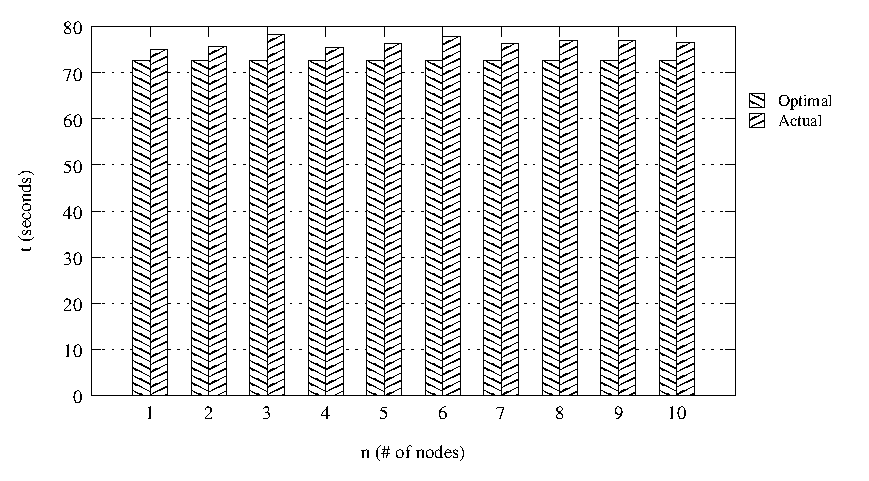
\epsfig{width=3.2in, angle=0, file=fig/grep.eps}
\caption{Grep experiment}
\label{fig:grepexperiment}
\end{figure}

\subsection{Sort}

We implemented a DataSeries program that sorts a distributed file. To implement the sort program, we hooked up the following
modules: $\tt SourceModule$, $\tt NetworkModule$ and $\tt
SortModule$.

For the experiment, we created data using $\tt gensort$, the random
data generator of the standard Sort Benchmark \cite{sortbenchmark}. (Each record
consist of a 10-byte key and a 90-byte value.) We ran the computation first on
a single-node ($n = 1$), and then on increasing cluster sizes ($n = 2, \ldots,
10$). For each cluster size $n$, we created a file of size $n \times 1$ GB,
and divided the file into $n$ equal partitions. We converted each partition to
the DataSeries format via $\tt gensort2ds$, a tool that converts
gensort-generated files to DataSeries files by creating one DataSeries record,
consisting of two fields (of type $\tt FixedWidthField$), key and value, for
each gensort record.

It is worth noting that we used in-memory sorting in these experiments.
As described previously, achieving pipelined parallelism with external sorting
requires two parallel in-memory sorting processes. Unfortunately, our automated
cluster installation system does not currently support 64-bit operating
systems, so we were constrained in the amount of memory available to our
programs (even though the nodes had sufficient physical memory).

\subsubsection{Disk-bound sort}

We first ran the sort experiment on the exact same cluster as the grep
experiment. Figure \ref{fig:sort1000experiment} shows the actual execution time along with the optimal
execution time (as predicted by our model). The execution time of PDS was
within 8-17\% of the optimal time.

Figure \ref{fig:sort1000experiment} also shows, for the actual and optimal
computations, how the time is divided between Phase 1 and Phase 2 (see Figure \ref{fig:mapreduce}). For the actual computation, the
figure also displays the time spent on the sort buckets phase (see
Figure \ref{fig:sort}), which we ignore in our model. The actual computation
also includes additional overhead that we do not attribute to
any of the three phases.

\begin{figure}
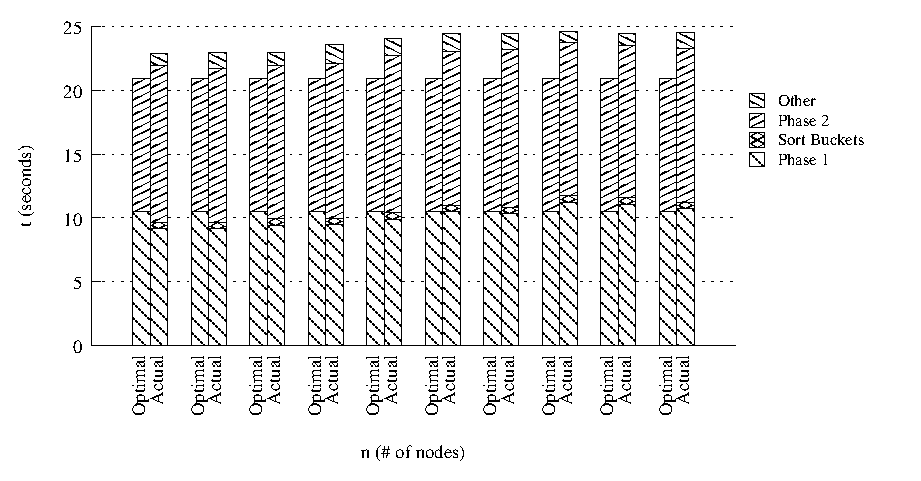
\epsfig{width=3.2in, angle=0, file=fig/sort1000.eps}
\caption{Disk-bound sort experiment}
\label{fig:sort1000experiment}
\end{figure}

\subsubsection{Network-bound sort}

To achieve a network-bound sort using our existing hardware, we
configured the network interfaces to negotiate only 100 Mb/s rather than 1 Gb/s. We also decreased the
MTU to 1500 bytes, the maximum supported by 100 Mbps Ethernet.

As with Figure \ref{fig:sort1000experiment}, Figure \ref{fig:sort100experiment}
shows, for the actual and optimal computations, how the time is divided between Phase 1 and Phase 2. The execution time in this experiment is much higher, due to the
constrained network bandwidth. The network does not affect the single-node
execution time, so it is very similar to that of the disk-bound sort
experiment. As the number of nodes increases, the execution time
grows. Even though the amount of input data per node is constant, the fraction
($\frac{n-1}{n}$) of the data that is sent over the network increases, because
the probability that any given input record is processed by the same node after
the partitioning becomes smaller. Also note that the time spent in Phase 2 is
not affected by the number of nodes, because Phase 2 does not include any
network-related activity.

\begin{figure}
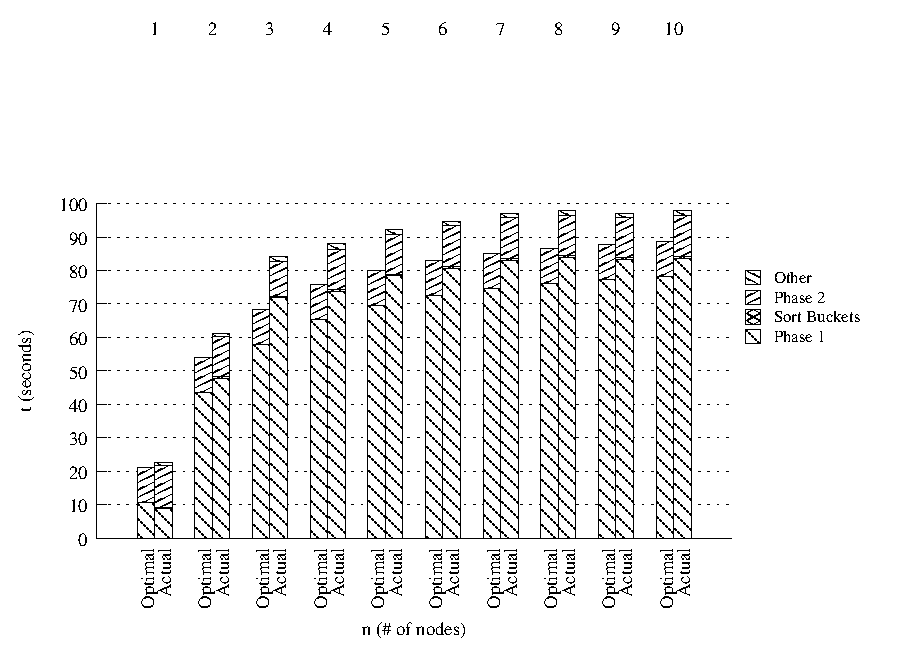
\epsfig{width=3.2in, angle=0, file=fig/sort100.eps}
\caption{Network-bound sort experiment}
\label{fig:sort100experiment}
\end{figure}

\section{Discussion and Future Work}

Our model, as outlined in Tables \ref{table:model1}, \ref{table:model2} and
\ref{table:model3}, take into account the per-node disk and network
throughputs. It does not consider, however, the network's backplane
bandwidth (aka switch fabric speed, bisection bandwidth). We believe that our
model, for several reasons. First, many clusters are used for multiple different
  computations in parallel. Rather than spreading computations accross a large
  number of nodes, it is possible to run each computation on a smaller,
  exclusive set of nodes, for which it is possible to provide full-speed
  all-to-all connectivity. In addition, many real-world applications do not need
  thousands of nodes. Such applications can run on smaller clusters that utilize a single switch
  (switches with hundreds of gigabit Ethernet ports, and full backplane
  bandwidth, are available from all of the major networking vendors).
  
We believe that parallel dataflow systems should consult an online model,
similar to the one described in this paper, when making scheduling decisions.
For example, the throughput of a map-reduce computation can increase
dramatically if the sorting can occur in memory, and in some cases this can be
achieved by scheduling the computation to run on a sufficient number of
nodes. For example, sorting 50 GB of data on 25 nodes would require
less machine-hours than sorting 50 GB on 10 nodes, assuming 4 GB of
RAM on each node. Furthermore, whether or not the first phase of a map-reduce
computation should include a backup write to disk depends on the execution time
of the computation. An online model could easily determine the expected
execution times (as a function of the other parameters), thereby allowing the
system to decide, at runtime, whether the system should perform backup writes.

\section{Related Work}
Google's MapReduce \cite{mapreduce} offers a programming model that enables
easy development of scalable parallel applications to process a vast amount of
data on large clusters of commodity machines. Through a simple interface with
two functions, map and reduce, this model facilitates parallel implementation
of many real-world tasks such as data processing and machine learning. Hadoop
\cite{hadoop} is an open-source map-reduce implementation for large clusters
that is very similar to \cite{mapreduce}. MapReduce and Hadoop, unlike PDS, are
highly inefficient due to various design and implementation details (eg,
exchanged data is always written to disk before it is sent over the network).

Phoenix \cite{phoenix} is a shared-memory implementation of the map-reduce
model for multi-core and SMP machines that allows programmers to develop
parallel applications without having to deal with threading and
synchronization. Due to its use of shared memory rather than temporary files
and TCP networking, Phoenix can  outperform MapReduce on a single machine.
Phoenix, unlike PDS, is designed to run only on a single machine.

Dryad \cite{dryad}, like MapReduce, offers a programming model and an execution
framework for writing parallel distributed programs. A Dryad programmer writes
several sequential programs and connects them using one-way channels. The
computation is structured as a directed graph (similarly to
\cite{paralleldatabases}). Dryad is responsible for executing the
user-specified graph on a cluster of commodity machines. Dryad also handles
fault tolerance, scheduling and resource management. Dryad is not publicly
available, and we were only able to find performance data for workloads that
involve very little data exchange.

Additional, higher-level languages have been introduced on top of MapReduce,
Hadoop and Dryad. These models further simplify the task of developing and
executing scalable parallel applications. Sawzall \cite{sawzall} is a
high-level language for the MapReduce framework that includes various built-in
aggregators. Pig Latin \cite{piglatin} is a high-level procedural language for
the Hadoop framework, which can also be executed on other frameworks (by
extending Pig, the compiler that translates Pig Latin programs into Hadoop
programs). Pig Latin offers various operators, such as COGROUP, FOREACH and
FILTER, and is similar to the declarative SQL language. DryadLINQ
\cite{dryadlinq} generates Dryad computations from the LINQ Language-Integrated
Query extensions to C\#. Programs written in Sawzall, Pig Latin and LINQ are
all translated to lower-level representations that can run on parallel dataflow
systems, and it should be possible to adapt them to support PDS.

Gordon \cite{gordon} is a system architecture for data-intensive applications
that combines low-power processors, flash memory and parallel dataflow systems
(eg, Hadoop) and improves the performance and power-consumption of such
applications. Gordon focuses on identifying the best hardware for large-scale
parallel processing. According to trace-based simulations (Gordon is not an
actual system), Gordon can outperform disk-based clusters by 1.5x. However, the
simulations do not account for networking, which is often the bottleneck in
such applications. Furthermore, Gordon assumes a given software stack and,
unlike PDS, does not address the relationship between the system's hardware and
software.

FAWN \cite{fawn} is a fast, scalable, and power-efficient cluster architecture
for data-intensive computing, and FAWNKV is a clustered key-value
storage system that runs on FAWN. Similar to Gordon, FAWN focuses on identifying
the best hardware for data-intensive computing, primarily in terms of queries
per joule.

\section{Conclusions}


We have proposed an analytical model for evaluating data-parallel programs and
parallel dataflow systems. This model will help developers and administrators
achieve higher performance and lower costs for data-intensive computing.
Developers will gain a better understanding of their bottlenecks, allowing them
to optimize the software in order to achieve better utilization of system
resources. Administrators will be able to acquire and deploy hardware that
provides a better balance among resources, thereby minimizing the
performance-cost ratio.

We have also described Parallel DataSeries (PDS), a
highly efficient parallel dataflow system that is capable of achieving
near-optimal performance. Through PDS, we have shown not only that it is
possible to achieve such efficiency, but also some of the important lessons and
techniques that enabled us to achieve this goal. We believe that by using
similar approaches, other systems can be modified to improve their efficiency.

%\end{document}  % This is where a 'short' article might terminate

%ACKNOWLEDGMENTS are optional
%\section{Acknowledgments}
%This section is optional; it is a location for you
%to acknowledge grants, funding, editing assistance and
%what have you.  In the present case, for example, the
%authors would like to thank Gerald Murray of ACM for
%his help in codifying this \textit{Author's Guide}
%and the \textbf{.cls} and \textbf{.tex} files that it describes.

%
% The following two commands are all you need in the
% initial runs of your .tex file to
% produce the bibliography for the citations in your paper.
\bibliographystyle{abbrv}
\bibliography{sigproc}  % sigproc.bib is the name of the Bibliography in this case
% You must have a proper ".bib" file
%  and remember to run:
% latex bibtex latex latex
% to resolve all references
%
% ACM needs 'a single self-contained file'!

\balancecolumns
% That's all folks!
\end{document}
